\appendix

%%%%%%%%%%%%%%%%%%%%%%%%%%%%%%%%%%%%%%%%%%%%%%%%%%%%%%%%%%%%%%%%%%%%%%%%
\section{Performance evaluation} \label{appendix:perf-eval}
%%%%%%%%%%%%%%%%%%%%%%%%%%%%%%%%%%%%%%%%%%%%%%%%%%%%%%%%%%%%%%%%%%%%%%%%

In this section we report additional performance measurements for \sys
to gauge how well it meets its goals.

\textbf{Methodology.} We recorded timestamps while our code is
executing using the Performance Web API\footnote{Note that while this
  API normally reports values as doubles, due to recent security
  threats, such as Spectre~\cite{DBLP:journals/corr/abs-1801-01203},
  several browser developers have implemented countermeasures by
  reducing the precision of the DOMHighResTimeStamp
  resolution~\cite{reducetimeprecision,resolutionconsiderations}. In
  particular, Firefox reports these values as integer
  milliseconds. For our tests, we re-enabled higher precision values.}

While our extension's functionality only applies at the network level,
there is potential slowdown at the DOM processing level due to the
optimization techniques the browser applies throughout several levels
of the web page load pipeline. \autoref{fig:navigationtiming} shows
the different timestamps provided by the Navigation Timing
API~\cite{navigationtiming}, as well as a high-level description of
the browser processing model. Since our filter listens on the
onBeforeRequest event, none of the previous steps before Request are
affected. In this section, we refer to the difference in time between
responseEnd and requestStart as the "network filter time".

\begin{figure}[h]
	\begin{center}
 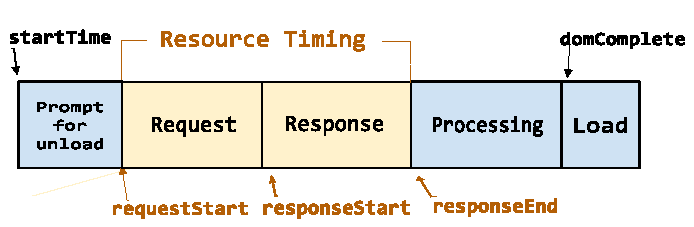
\includegraphics[scale=0.65]{img/timestamp-diagram-edited.pdf}
 \end{center}
 \caption{The Navigation Timing API's timestamps\protect\footnotemark}
 \label{fig:navigationtiming}
 \end{figure}

\footnotetext{This image was taken from the w3 spec: \url{https://www.w3.org/TR/navigation-timing-2/}}


\subsection{Top websites load times; continued} \label{top_sites}

\iffalse
\begin{figure}[h]
	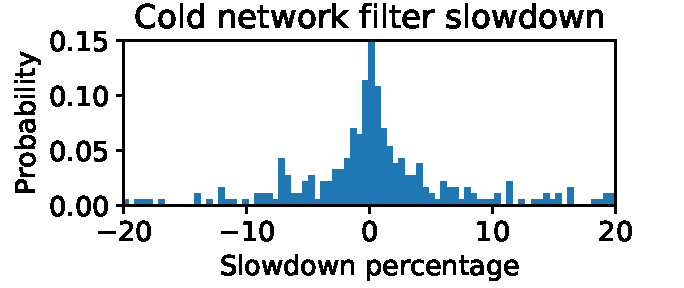
\includegraphics[scale=0.5]{results/density_histogram_filter_slowdown_small.pdf}
	\caption{Density histogram of network filter slowdown for top sites.}
	\label{fig:histogram_slowdown}
\end{figure}


Figure ~\ref{fig:histogram_slowdown} shows a closer look at the distribution for the cold network filter slowdown on the top sites (same values as in \autoref{fig:overall_slowdown}). For this component, 87.6\% of the slowdown values are less than 10\%.
\fi

\begin{figure}[h]
	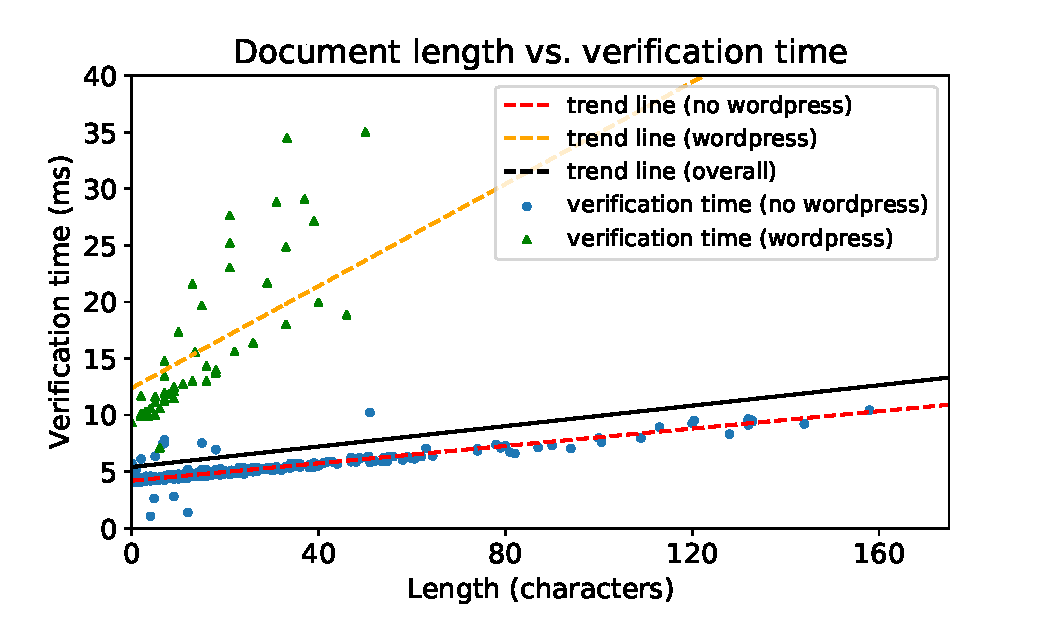
\includegraphics[scale=0.5]{results/string_length_vs_verification_time_small.pdf}
	\caption{Scatter plot of network filter time as a function of character length for top sites.}
	\label{fig:verification_time_string_length}
\end{figure}

 \autoref{fig:verification_time_string_length} shows the time spent by the call to our string verification function in the network filter as a function of the length of the string to be verified. The blue dots are the pages for which our framework probes tested negative, and the green triangles are the pages for which the probes tested positive: 55 in total. We applied least squares regression to calculate the shown trend lines. The Spearman's rank \footnote{The Spearman's correlation coefficient measures the strength and direction of association between two ranked variables: https://statistics.laerd.com/statistical-guides/spearmans-rank-order-correlation-statistical-guide.php} correlation values for no probe, probe, and overall are 0.91, 0.91, and 0.72 respectively, demonstrating positive correlation. Since both our probes and signatures use regex matching, we expect both trend lines to be linear, as seen in the graph. Recall that once a probe for a certain software passes, we perform a linear scan over the signatures for that specific software and check whether it applies to the given HTML string or not. Thus, we expect the slope of the line to be higher when a probe passes. Around 37.4\% of all web sites use frameworks covered by our probes~\cite{w3stats}, thus, we expect the impact of our network filter to be closer to the non-probe values, as corroborated by our overall trend line.
 

\textbf{False positives on the Web.} Additionally, for each website, we recorded the number of loaded signatures. We report a 0\% FP rate for loaded signatures. Thus, we can infer with confidence that the rate of false positives for loaded signatures during an average user's web browsing is similarly low. This rate could possibly go up as the number of signatures and covered frameworks increases. It is likely that these websites are free of vulnerabilities covered by our signatures, as many of these websites are not running WordPress to begin with, and being the most popular, they would likely be updated quickly if a vulnerability is found; thus, the rate of false negatives is likely extremely low as well.

\subsection{WordPress websites load times} \label{wordpress_sites}

We ran similar experiments as in Section 6.1, but with the WordPress sites described in Section 4.1. Thus, all of these have either one or multiple injection points in their HTML, and the network filter will spend an additional amount of time sanitizing these as defined by the signatures. Note that the data set is smaller here, and some of the trends might be harder to infer.

\autoref{fig:WordPress_slowdown} shows the results for slowdown with the extension running for these sites. Recall that the only difference between a page which passes the WordPress probe and one that matches a signature is that the latter has to replace a portion of the original string by its sanitized version. In this case we see a slowdown of less than 10\% for 60\% of sites, and less than 40\% for 96.25\% of them. The warm network filter curve suffers from a particularly high slowdown. We believe this to be the case because the locally hosted pages decrease the network component time, causing any overhead to be seen as relatively high. However, as 48\% of the original values were below 60ms, conclude a small impact on user experience as well.

\begin{figure}[h]
	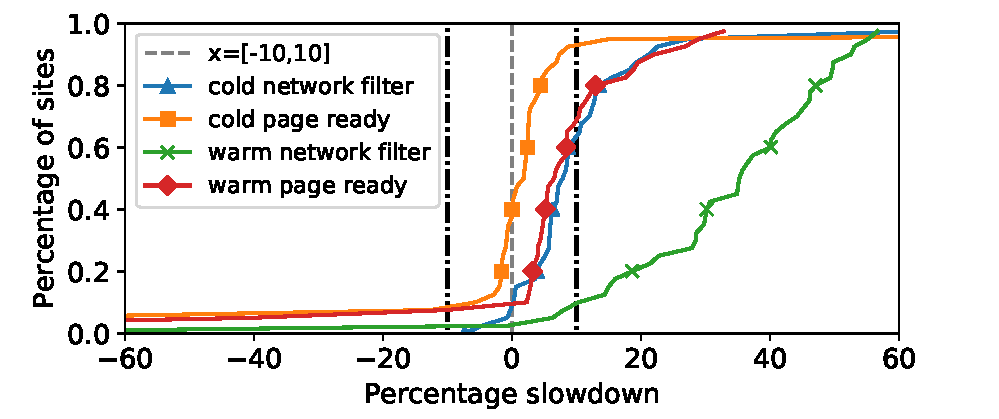
\includegraphics[scale=0.5]{results/extension_slowdown_wordpress_small.pdf}
	\caption{Cumulative distribution of relative percentage slowdown with extension installed for WordPress sites.}
	\label{fig:WordPress_slowdown}
\end{figure}

\iffalse
\autoref{fig:histogram_slowdown_wordpress} shows the probability density of the cold network filter slowdown. In this case, we see that the distribution is skewed more towards a higher slowdown. As it is harder to discern the trend for this data set than its top site counterpart, we have also plotted the normal distribution of the data between 3 standard deviations. 65\% of values are less than 10\%.

\begin{figure}[h]
	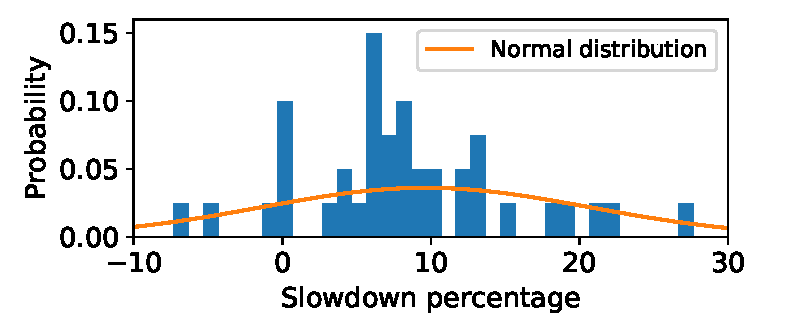
\includegraphics[scale=0.5]{results/density_histogram_filter_slowdown_wordpress_small.pdf}
	\caption{Density histogram of network filter slowdown for WordPress sites.}
	\label{fig:histogram_slowdown_wordpress}
\end{figure}
\fi

Finally, we report the string verification time as a function of its length, for the WordPress sites, shown in \autoref{fig:verification_time_string_length_wordpress}. The Spearman's rank correlation for this set of data is 0.630.


\begin{figure}[h]
	\begin{center}
	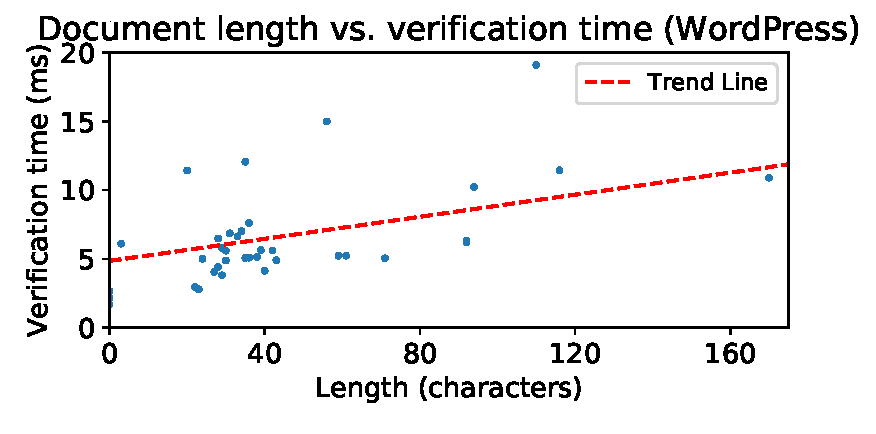
\includegraphics[scale=0.55]{results/string_length_vs_verification_time_wordpress_small.pdf}
	
	\caption{Scatter plot of network filter time as a function of character length for WordPress sites.}
	\label{fig:verification_time_string_length_wordpress}
\end{center}
\end{figure}




%% %%%%%%%%%%%%%%%%%%%%%%%%%%%%%%%%%%%%%%%%%%%%%%%%%%%%%%%%%%%%%%%%%%%%%%%%
%% \section{Signature Language Specification} \label{appendix:language_specification}
%% %%%%%%%%%%%%%%%%%%%%%%%%%%%%%%%%%%%%%%%%%%%%%%%%%%%%%%%%%%%%%%%%%%%%%%%%

%% We provide a description of our signature language, in particular in the context of WordPress:
%% \begin{itemize}
%% 	\item
%% 	url: If the exploit occurs in a specific URL or subdomain, this is defined as a string, e.g.
%% 	\url{/wp-admin/options-general.php?page=relevanssi\%2Frelevanssi.php}, otherwise null.
%% 	\item
%% 	software: The software framework the page is running if any, e.g. WordPress. A hand-crafted page
%% 	might not have any identifiable software.
%% 	\item
%% 	softwareDetails: If running any software, this provides further information about when to load a signature. For WordPress, these are plugin names as depicted in the HTML of a page running such plugin.
%% 	\item
%% 	version: The version number of the software/plugin/page. This is used for versioning of the software run by the page, as described in \autoref{versioning}.
%% 	\item 
%% 	type: A string describing the signature type. A value of "string" describes a basic signature. A value of 'listener' describes a signature which requires an additional listener in the background page for network requests.
%% 	\item 
%% 	sanitizer: A string with one of the following values: "DOMPurify", "escape", and "regex". This item is optional, the default is DOMPurify.
%% 	\item
%% 	config: The config parameters to go along with the chosen sanitizer, if necessary. For "DOMPurify", the accepted values are as defined by the DOMPurify API (i.e, DOMPurify.sanitize(dirty, config). For "escape", an additional escaping pattern can be provided. For "regex", this should be the pattern to match with the injection point content.
%% 	\item
%% 	typeDet: A string with the following pattern: 'occurrence-uniqueness'. As described in Section 2.4, this specifies whether there are several injection points in the HTML.
%% 	\item
%% 	endPoints: An array of startpoint and endpoint tuples.
%% 	\item 
%% 	endPointsPositions: An array of integer tuples. These are optional but useful when the one of the endPoints HTML are used throughout the whole page and appear a fixed number of times. For example: if an injection ending point happens on an element <h3 class='my-header'>, this element might have 10 appearances throughout the page. However, only the 4th is an injection ending point. The signature would specify the second element of the tuple to be 7, as it would be the 7th such item in a regex match array (using 1-based indexing), counting from the bottom up. For ending points, we have to count from the bottom up because the attacker can inject arbitrarily many of these elements before it, and vice versa for starting points.
%% \end{itemize}

%% Additionally, if the value of type is `listener', the signature will have an additional field called listenerData. Similarly to a regular signature, this consists of the following pieces of information:
%% \begin{itemize}
%% 	\item 
%% 	listenerType: The type of network listener as defined by the WebRequest API (e.g. `script', `XHR', etc.)
%% 	\item
%% 	listenerMethod: The request's HTTP method, for example "GET" or "POST".
%% 	\item
%% 	url: the URL of the request target.
%% \end{itemize}
